%\documentclass[
  bibliography=totoc,     % Literatur im Inhaltsverzeichnis
  captions=tableheading,  % Tabellenüberschriften
  titlepage=firstiscover, % Titelseite ist Deckblatt
]{scrartcl}

% Paket float verbessern
\usepackage{scrhack}

% Warnung, falls nochmal kompiliert werden muss
\usepackage[aux]{rerunfilecheck}

% unverzichtbare Mathe-Befehle
\usepackage{amsmath}
% viele Mathe-Symbole
\usepackage{amssymb}
% Erweiterungen für amsmath
\usepackage{mathtools}

% Fonteinstellungen
\usepackage{fontspec}
% Latin Modern Fonts werden automatisch geladen
% Alternativ zum Beispiel:
%\setromanfont{Libertinus Serif}
%\setsansfont{Libertinus Sans}
%\setmonofont{Libertinus Mono}

% Wenn man andere Schriftarten gesetzt hat,
% sollte man das Seiten-Layout neu berechnen lassen
\recalctypearea{}

% deutsche Spracheinstellungen
\usepackage[ngerman]{babel}


\usepackage[
  math-style=ISO,    % ┐
  bold-style=ISO,    % │
  sans-style=italic, % │ ISO-Standard folgen
  nabla=upright,     % │
  partial=upright,   % │
  mathrm=sym,        % ┘
  warnings-off={           % ┐
    mathtools-colon,       % │ unnötige Warnungen ausschalten
    mathtools-overbracket, % │
  },                       % ┘
]{unicode-math}

% traditionelle Fonts für Mathematik
\setmathfont{Latin Modern Math}
% Alternativ zum Beispiel:
%\setmathfont{Libertinus Math}

\setmathfont{XITS Math}[range={scr, bfscr}]
\setmathfont{XITS Math}[range={cal, bfcal}, StylisticSet=1]

% Zahlen und Einheiten
\usepackage[
  locale=DE,                   % deutsche Einstellungen
  separate-uncertainty=true,   % immer Unsicherheit mit \pm
  per-mode=symbol-or-fraction, % / in inline math, fraction in display math
]{siunitx}

% chemische Formeln
\usepackage[
  version=4,
  math-greek=default, % ┐ mit unicode-math zusammenarbeiten
  text-greek=default, % ┘
]{mhchem}

% richtige Anführungszeichen
\usepackage[autostyle]{csquotes}

% schöne Brüche im Text
\usepackage{xfrac}

% Standardplatzierung für Floats einstellen
\usepackage{float}
\floatplacement{figure}{htbp}
\floatplacement{table}{htbp}

% Floats innerhalb einer Section halten
\usepackage[
  section, % Floats innerhalb der Section halten
  below,   % unterhalb der Section aber auf der selben Seite ist ok
]{placeins}

% Seite drehen für breite Tabellen: landscape Umgebung
\usepackage{pdflscape}

% Captions schöner machen.
\usepackage[
  labelfont=bf,        % Tabelle x: Abbildung y: ist jetzt fett
  font=small,          % Schrift etwas kleiner als Dokument
  width=0.9\textwidth, % maximale Breite einer Caption schmaler
]{caption}
% subfigure, subtable, subref
\usepackage{subcaption}

% Grafiken können eingebunden werden
\usepackage{graphicx}

% schöne Tabellen
\usepackage{tabularray}
\UseTblrLibrary{booktabs, siunitx}

% Verbesserungen am Schriftbild
\usepackage{microtype}

% Literaturverzeichnis
\usepackage[
  backend=biber,
]{biblatex}
% Quellendatenbank
\addbibresource{lit.bib}
\addbibresource{programme.bib}

% Hyperlinks im Dokument
\usepackage[
  german,
  unicode,        % Unicode in PDF-Attributen erlauben
  pdfusetitle,    % Titel, Autoren und Datum als PDF-Attribute
  pdfcreator={},  % ┐ PDF-Attribute säubern
  pdfproducer={}, % ┘
]{hyperref}
% erweiterte Bookmarks im PDF
\usepackage{bookmark}

% Trennung von Wörtern mit Strichen
\usepackage[shortcuts]{extdash}

\author{%
  Vincent Wirsdörfer\\%
  \href{mailto:vincent.wirsdoerfer@udo.edu}{authorA@udo.edu}%
  \and%
  Joris Daus\\%
  \href{mailto:joris.daus@udo.edu}{authorB@udo.edu}%
}
\publishers{TU Dortmund – Fakultät Physik}


%\begin{document}
\section{Diskussion}
\label{sec:Diskussion}

Zu Beginn ist zu erwähnen, dass die Werte nicht selbst aufgenommen worden sind. Es kann somit nicht darauf eingegangen werden, was 
bei der Messung ggf. schiefgegangen ist. Es können lediglich die vorhandenen Messwerte auf ihre Plausibilität überprüft werden. \\
\noindent Der Verlauf der blauen Photostrom-Kennlinien entspricht den Erwartungen aus der Theorie, jedoch sollte der Verlauf bei 
der halben Intensität auch nur die Hälfte des Maximums der vollen Intensität besitzen. Dies ist nicht der Fall. Es ist in der Tat 
sogar das Gegenteil der Fall, sodass die Intensität der zweiten Linie mit geringerer Spaltbreite eine höhere Intensität besitzt als 
die mit größerer Spaltbreite. Dies lässt sich nur durch einen systematischen Fehler erklären. \\

Für die Grenzspannungen gibt es keinen Literaturwert, da dies ein Wert ist, welcher von dem Versuchsaufbau abhängt. Die berechneten 
Werte stimmen jedoch in etwa mit den abgelesenen Werten überein. Sodass gesagt werden kann, dass die Rechnung zuverlässige 
Ergebnisse liefert. Auch der Fakt, dass das gelbe Licht perfekt in einer gerade liegt, deutet auf zuverlässige Daten hin.\\
\noindent Die Auftragung der verschiedenen Grenzspannungen ergibt auf den ersten Blick bereits eine Gerade. Der Fit bestätigt 
diese Vermutung. In \autoref{fig:Planck} und \autoref{fig:Planck_read} wird bereits der Theoriewert für die Planckkonstante als 
Steigung angenommen, um einen Vergleich zu schaffen. Dabei ist zu sehen, dass der Theoriewert sehr dich am gemessenen Wert dran ist. 
In der Tat weichen die berechneten Planckkonstanten vom Literaturwert \qty{4.135e-15}{e \volt \second} \cite{Planck} nur wenig ab: 

\begin{align*}
    \Delta{}h_\text{berechnet} &= 3.7\pm1.2 \\
    \Delta{}h_\text{abgelesen} &= 3.3\pm1.6
\end{align*}

\noindent Die ermittelte Austrittsarbeit liegt mit 

\begin{align*}
    \Phi_\text{berechnet} &= \qty{1.62\pm0.03}{e \volt}\\
    \Phi_\text{abgelesen} &= \qty{1.63\pm0.04}{e \volt}
\end{align*}

\noindent weit von der Austrittsarbeit von Silber mit \qty{4.5\pm0.24}{e \volt}\cite{Austrittsarbeit}. Die Austrittsarbeit ist jedoch 
im Bereich von der von Calciumoxid mit \qty{1.6\pm0.2}{e \volt}. Dies kann daran liegen, dass das Kalium verunreinigt ist und z.B. 
mit Silberoxid vermischt wurde. Auch Fremdmaterialien können die Messung verfälschen. 

\section{Anhang}

\begin{figure}
    \centering
    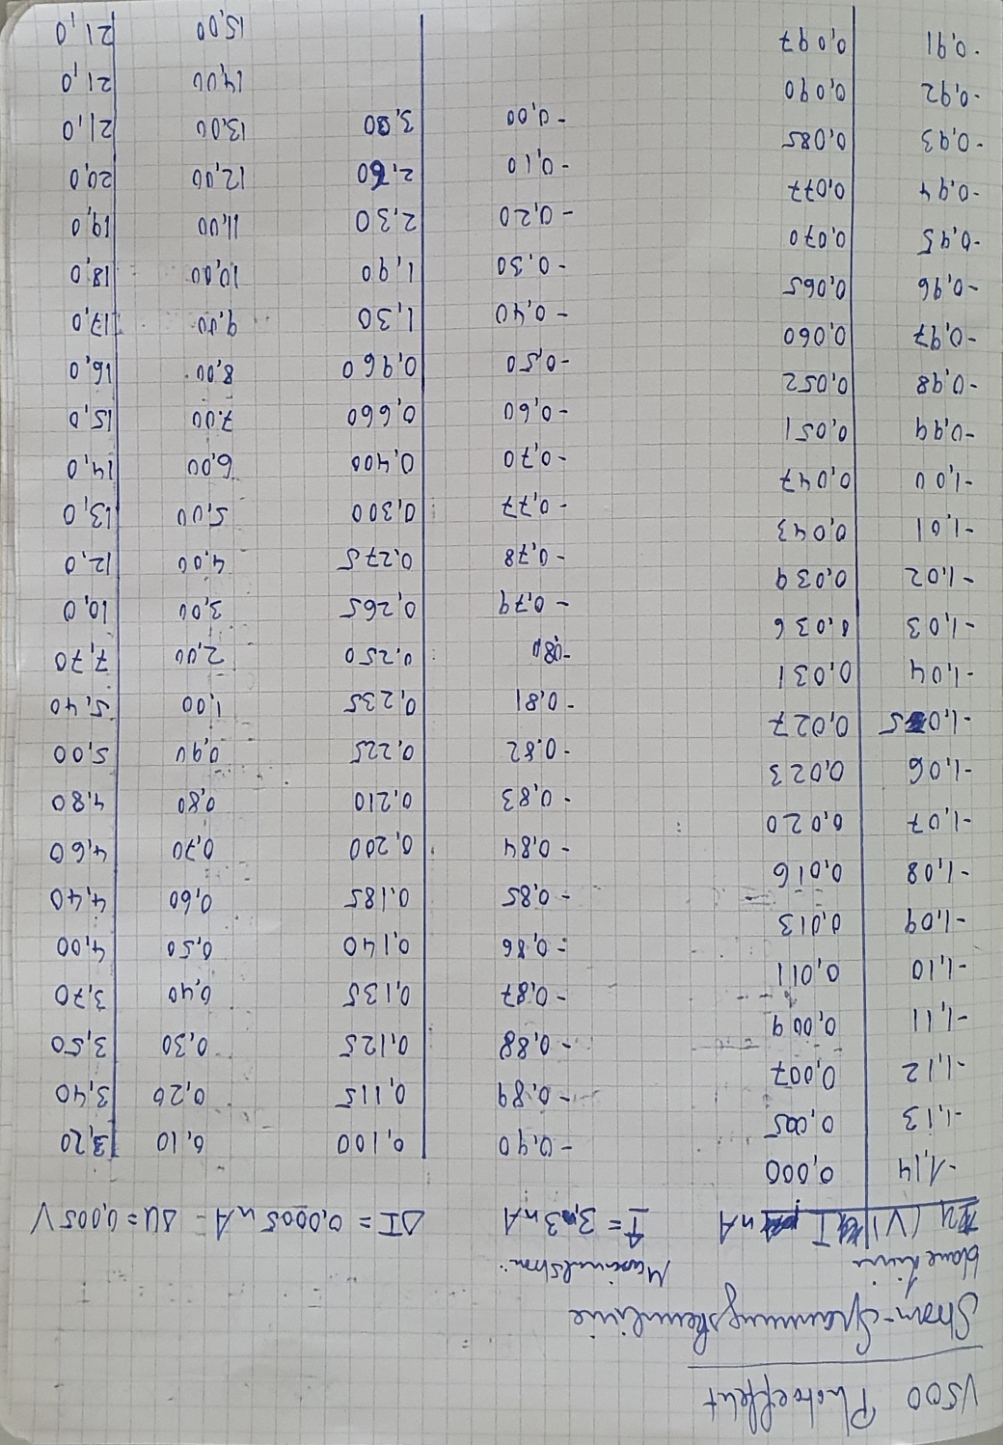
\includegraphics[width=0.9\textwidth]{content/Laborbuch_voll.jpg}
    \caption{Messdaten des blauen Lichts bei voller Intensität.}
\end{figure}

\begin{figure}
    \centering
    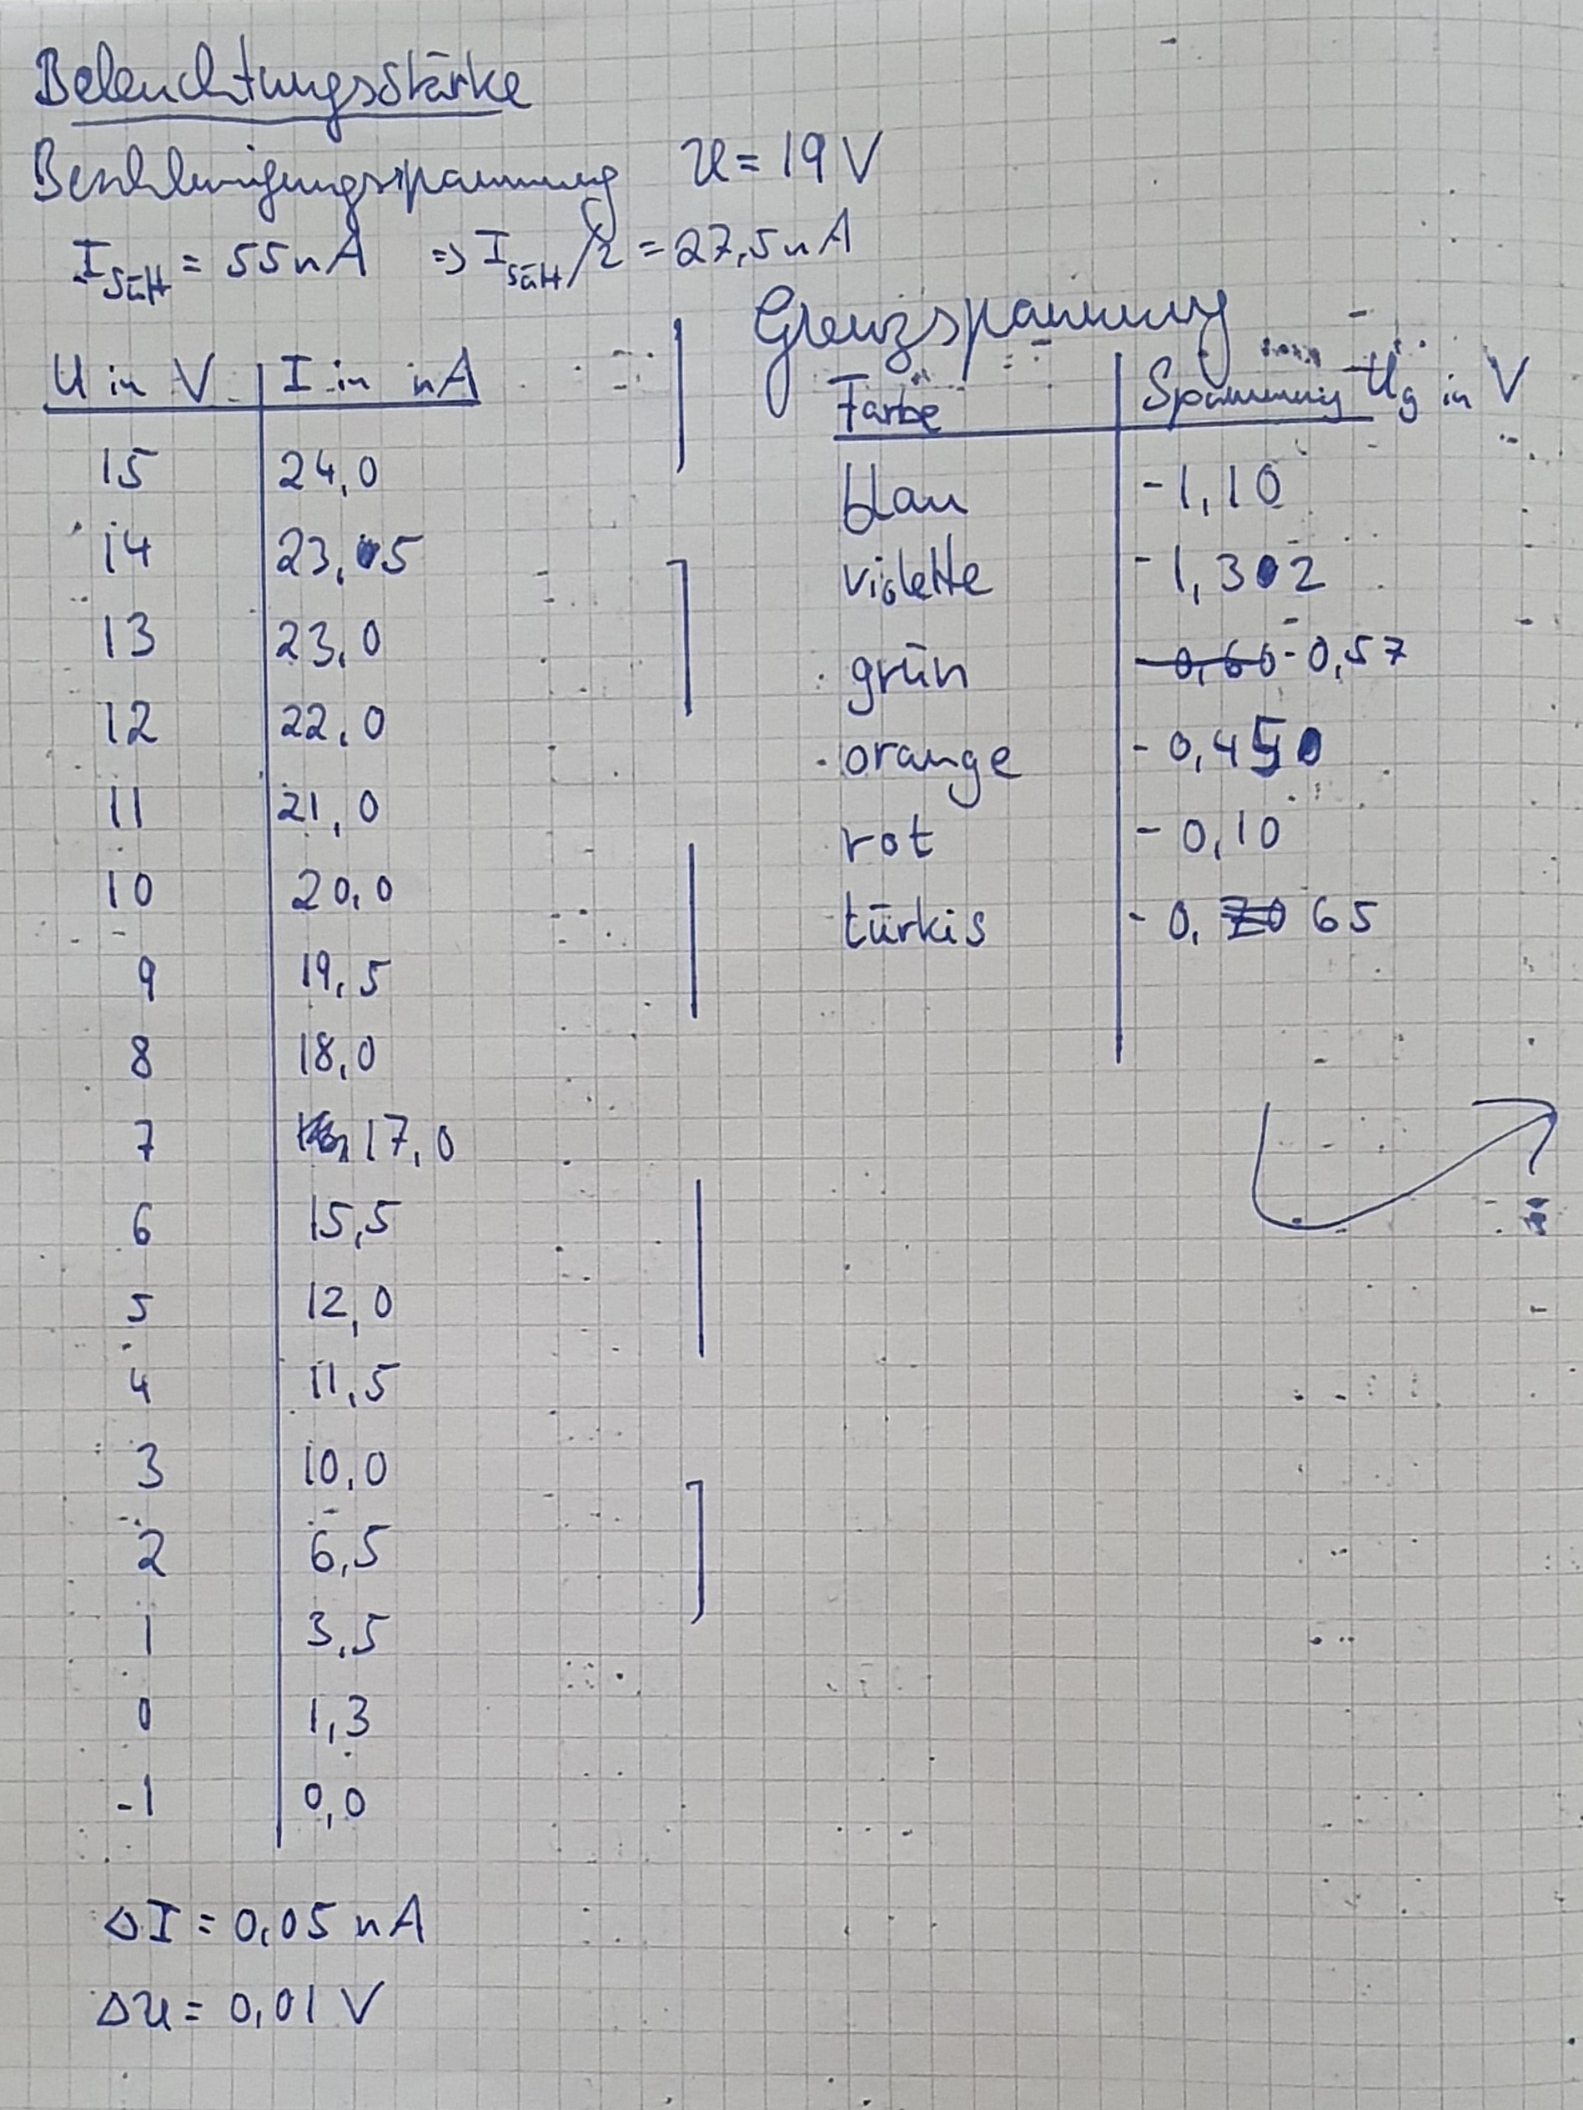
\includegraphics[width=0.9\textwidth]{content/Laborbuch_halb.jpg}
    \caption{Messdaten des blauen Lichts bei halber Intensität.}
\end{figure}

\begin{figure}
    \centering
    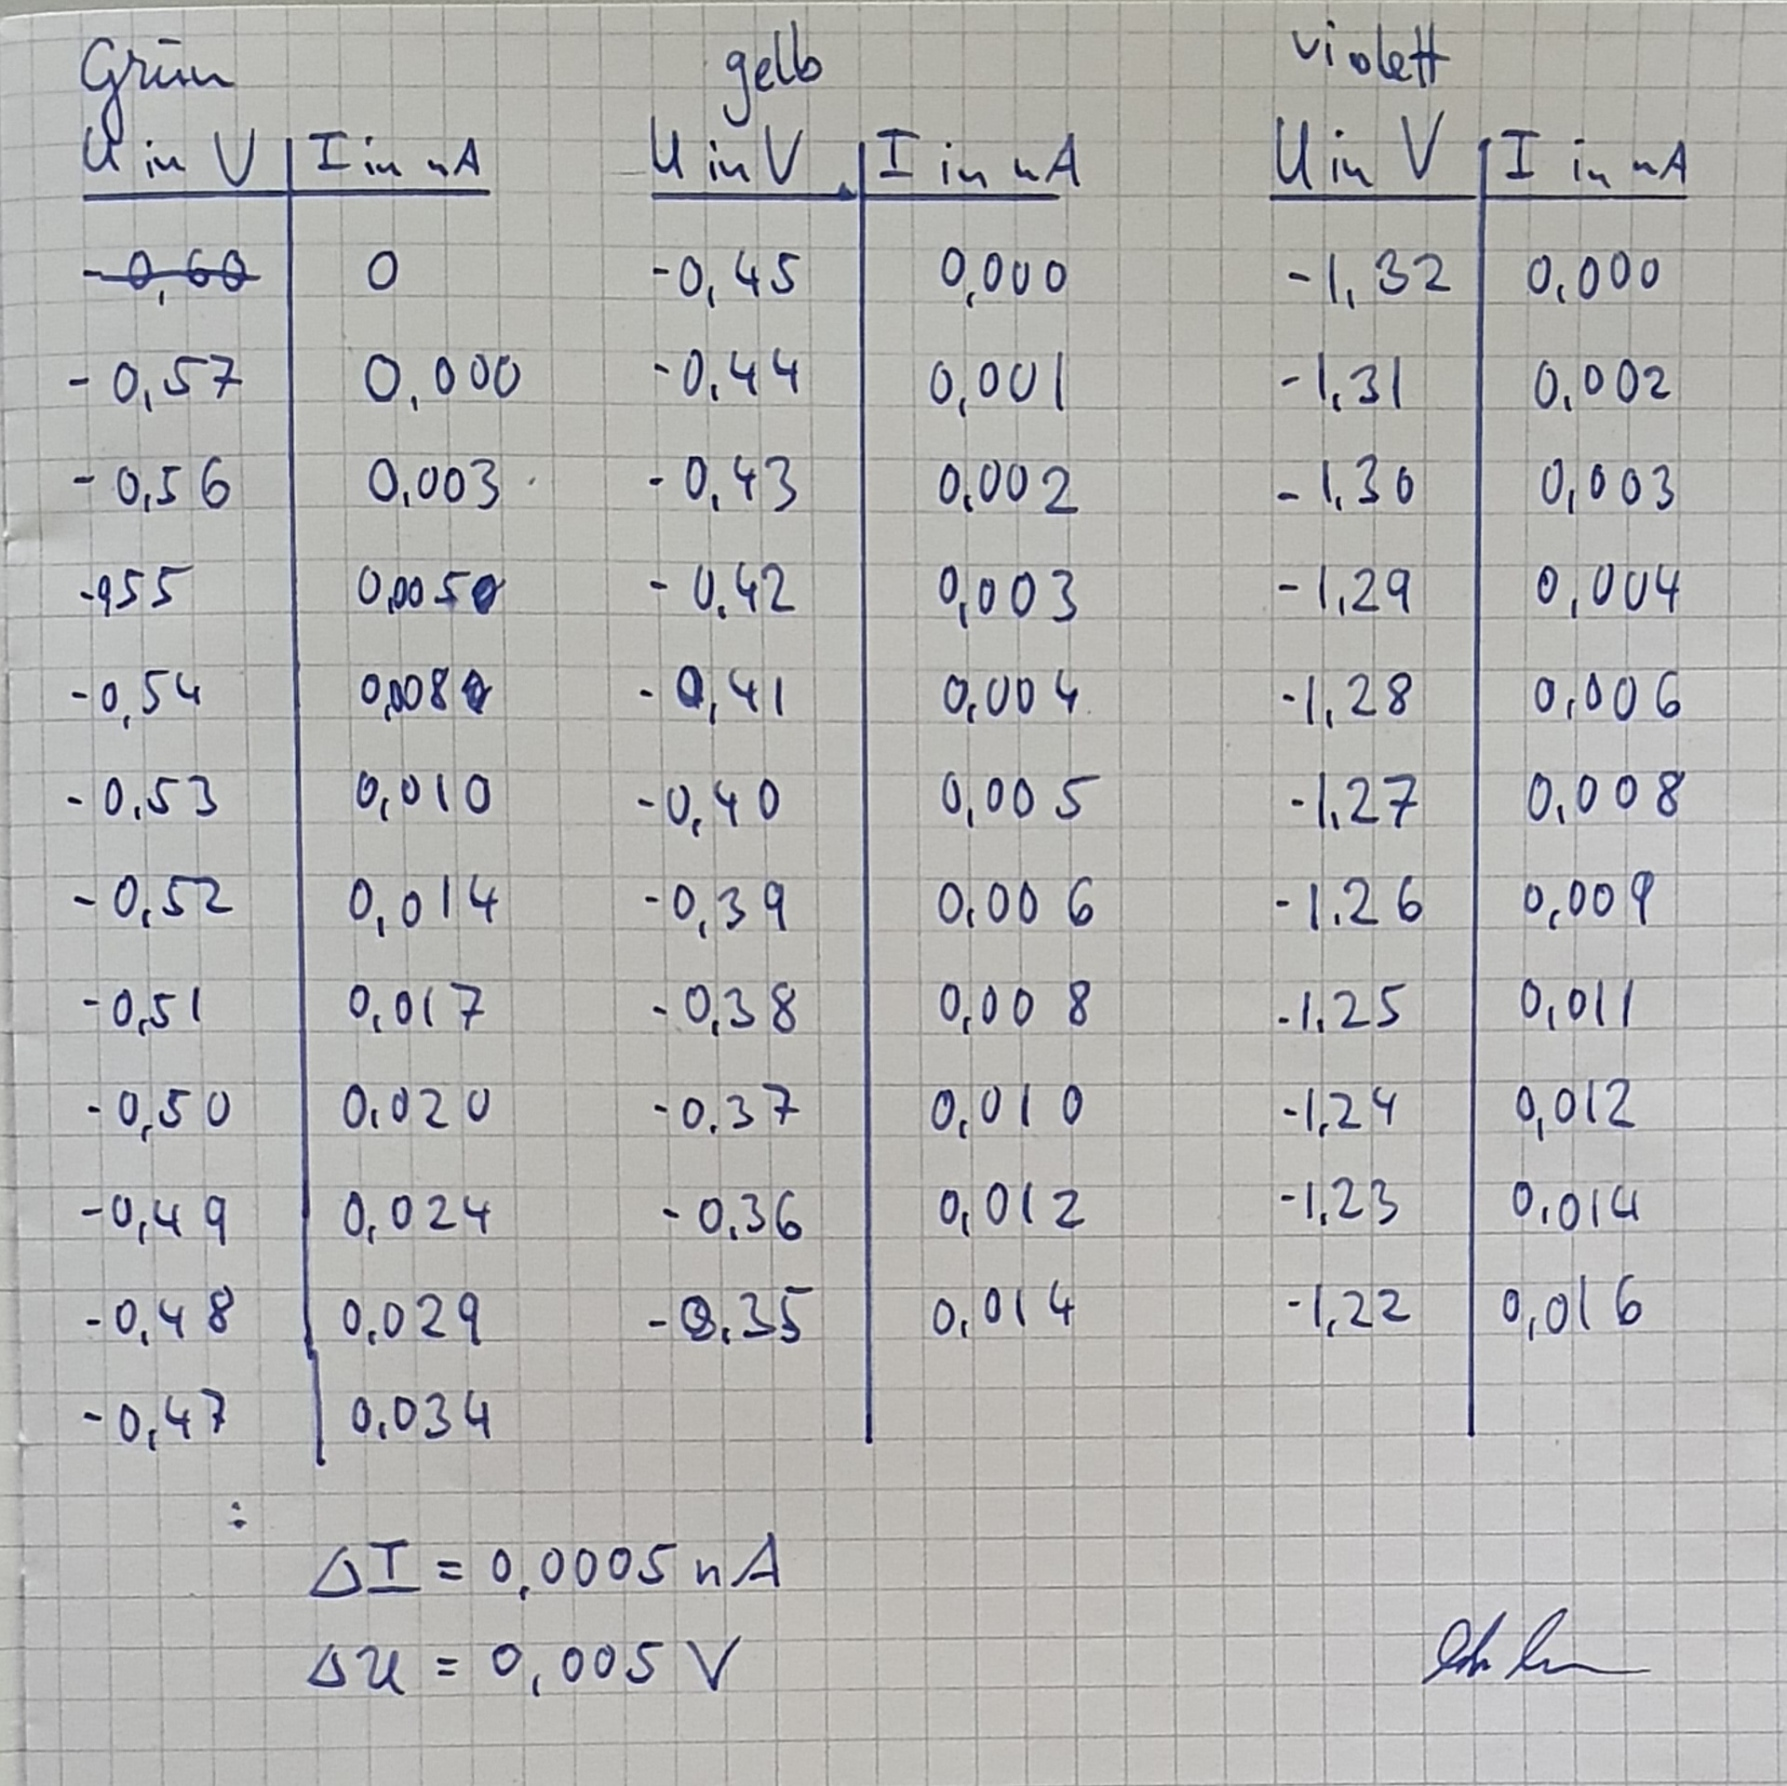
\includegraphics[width=0.9\textwidth]{content/Laborbuch_bunt.jpg}
    \caption{Messdaten des gelben, grünen und violetten Lichts bei halber Intensität.}
\end{figure}

%\end{document}
